%% LyX 2.3.4.2 created this file.  For more info, see http://www.lyx.org/.
%% Do not edit unless you really know what you are doing.
\documentclass[11pt,american,czech]{book}
\usepackage[T1]{fontenc}
\usepackage[utf8]{inputenc}
\usepackage[a4paper]{geometry}
\geometry{verbose,tmargin=4cm,bmargin=3cm,lmargin=3cm,rmargin=2cm,headheight=0.8cm,headsep=1cm,footskip=0.5cm}
\pagestyle{headings}
\setcounter{secnumdepth}{3}
\usepackage{url}
\usepackage{amsmath}
\usepackage{amsthm}
\usepackage{amssymb}
\usepackage{graphicx}
\usepackage{setspace}
\usepackage{xcolor}

\newtheorem{definition}{Definice}[chapter]
\newtheorem{lemma}{Lemma}[chapter]
\newtheorem{theorem}{Tvrzení}[chapter]
\newtheorem{corollary}{Důsledek}[chapter]
\newtheorem{remark}{Poznámka}[chapter]
\newtheorem{dukaz}{Důkaz}
\newtheorem{veta}{Věta}

\makeatletter
%%%%%%%%%%%%%%%%%%%%%%%%%%%%%% Textclass specific LaTeX commands.
\newenvironment{lyxlist}[1]
	{\begin{list}{}
		{\settowidth{\labelwidth}{#1}
		 \setlength{\leftmargin}{\labelwidth}
		 \addtolength{\leftmargin}{\labelsep}
		 \renewcommand{\makelabel}[1]{##1\hfil}}}
	{\end{list}}

\usepackage{graphicx}
\graphicspath{ {./Images/} }

%%%%%%%%%%%%%%%%%%%%%%%%%%%%%% User specified LaTeX commands.
%% Font setup: please leave the LyX font settings all set to 'default'
%% if you want to use any of these packages:

%% Use Times New Roman font for text and Belleek font for math
%% Please make sure that the 'esint' package is turned off in the
%% 'Math options' page.
\usepackage[varg]{txfonts}

%% Use Utopia text with Fourier-GUTenberg math
%\usepackage{fourier}

%% Bitstream Charter text with Math Design math
%\usepackage[charter]{mathdesign}

%%---------------------------------------------------------------------

%% Make the multiline figure/table captions indent so that the second
%% line "hangs" right below the first one.
%\usepackage[format=hang]{caption}

%% Indent even the first paragraph in each section
\usepackage{indentfirst}
\usepackage[LGRgreek]{mathastext}

%%---------------------------------------------------------------------

%% Disable page numbers in the TOC. LOF, LOT (TOC automatically
%% adds \thispagestyle{chapter} if not overriden
%\addtocontents{toc}{\protect\thispagestyle{empty}}
%\addtocontents{lof}{\protect\thispagestyle{empty}}
%\addtocontents{lot}{\protect\thispagestyle{empty}}

%% Shifts the top line of the TOC (not the title) 1cm upwards 
%% so that the whole TOC fits on 1 page. Additional page size
%% adjustment is performed at the point where the TOC
%% is inserted.
%\addtocontents{toc}{\protect\vspace{-1cm}}

%%---------------------------------------------------------------------

% completely avoid orphans (first lines of a new paragraph on the bottom of a page)
\clubpenalty=9500

% completely avoid widows (last lines of paragraph on a new page)
\widowpenalty=9500
\setlength{\parskip}{1em}

% disable hyphenation of acronyms
\hyphenation{CDFA HARDI HiPPIES IKEM InterTrack MEGIDDO MIMD MPFA DICOM ASCLEPIOS MedInria}

%%---------------------------------------------------------------------

%% Print out all vectors in bold type instead of printing an arrow above them
\renewcommand{\vec}[1]{\boldsymbol{#1}}

% Replace standard \cite by the parenthetical variant \citep
%\renewcommand{\cite}{\citep}

\makeatother
\usepackage{enumitem}



\usepackage{babel}
\begin{document}
\def\documentdate{7. \v{c}ervence 2020}

%%\def\documentdate{\today}

\pagestyle{empty}
{\centering

\noindent %
\begin{minipage}[c]{3cm}%
\noindent \begin{center}

\includegraphics[width=3cm,height=3cm,keepaspectratio]{Images/TITLE/cvut}
\par\end{center}%
\end{minipage}%
\begin{minipage}[c]{0.6\linewidth}%
\begin{center}
\textsc{\large{}České vysoké učení technické v Praze}{\large{}}\\
{\large{}Fakulta jaderná a fyzikálně inženýrská}
\par\end{center}%
\end{minipage}%
\begin{minipage}[c]{3cm}%
\noindent \begin{center}

\includegraphics[width=3cm,height=3cm,keepaspectratio]{Images/TITLE/fjfi}
\par\end{center}%
\end{minipage}

\vspace{3cm}

\textbf{\huge{}Využití prediktorů pro odhadování parametrů}{\huge\par}

\vspace{1cm}

\selectlanguage{american}%
\textbf{\huge{}Exploitation of predictors for parameter estimation}{\huge\par}

\selectlanguage{czech}%
\vspace{2cm}

{\large{}Výzkumný úkol}{\large\par}

}

\vfill{}

\begin{lyxlist}{MMMMMMMMM}
\begin{singlespace}
\item [{Autor:}] \textbf{Yana Podlesna}
\item [{Vedoucí~práce:}] \textbf{Ing. Miroslav Kárný, DrSc.}
\item [{Akademický~rok:}] 2020/2021
\end{singlespace}
\end{lyxlist}
\newpage{}

~\newpage{}

~

\vfill{}

\begin{center}
- Zadání práce -
\par\end{center}

\vfill{}

~\newpage{}

~

\vfill{}

\begin{center}
- Zadání práce (zadní strana) -
\par\end{center}

\vfill{}

~\newpage{}

\noindent \emph{\Large{}Poděkování:}{\Large\par}

\noindent Chtěl bych zde poděkovat především svému školiteli ...................
za pečlivost, ochotu, vstřícnost a odborné i lidské zázemí při vedení
mé diplomové práce. Dále děkuji svému konzultantovi ................
za ................

\vfill

\noindent \emph{\Large{}Čestné prohlášení:}{\Large\par}

\noindent Prohlašuji, že jsem tuto práci vypracoval samostatně a uvedl
jsem všechnu použitou literaturu.

\bigskip{}

\noindent V Praze dne \documentdate\hfill{} Yana Podlesna

\vspace{2cm}

\newpage{}

~\newpage{}

\begin{onehalfspace}
\noindent \emph{Název práce:}

\noindent \textbf{ Využití prediktorů pro odhadování parametrů}
\end{onehalfspace}

\bigskip{}

\noindent \emph{Autor:} Yana Podlesna

\bigskip{}

\noindent \emph{Obor:} Celý název oboru (nikoliv zkratka)\bigskip{}

\noindent \emph{Zaměření:} Celý název zaměření (Pokud obor neobsahuje
zaměření, tuto řádku odstranit.)

\bigskip{}

\noindent \emph{Druh práce:} Výzkumný úkol

\bigskip{}

\noindent \emph{Vedoucí práce:} Ing. Miroslav Kárný, DrSc.,
pracoviště školitele (název instituce, fakulty, katedry...)

\bigskip{}

\noindent \emph{Konzultant:} doc. RNDr. Jméno Konzultanta, CSc., pracoviště
konzultanta. Pouze pokud konzultant byl jmenován.

\bigskip{}

\noindent \emph{Abstrakt:} Abstrakt max. na 10 řádků. Abstrakt max.
na 10 řádků. Abstrakt max. na 10 řádků. Abstrakt max. na 10 řádků.
Abstrakt max. na 10 řádků. Abstrakt max. na 10 řádků. Abstrakt max.
na 10 řádků. Abstrakt max. na 10 řádků. Abstrakt max. na 10 řádků.
Abstrakt max. na 10 řádků. Abstrakt max. na 10 řádků. Abstrakt max.
na 10 řádků. Abstrakt max. na 10 řádků. Abstrakt max. na 10 řádků.
Abstrakt max. na 10 řádků. Abstrakt max. na 10 řádků. Abstrakt max.
na 10 řádků. Abstrakt max. na 10 řádků. Abstrakt max. na 10 řádků.
Abstrakt max. na 10 řádků. Abstrakt max. na 10 řádků. Abstrakt max.
na 10 řádků. Abstrakt max. na 10 řádků. Abstrakt max. na 10 řádků.
Abstrakt max. na 10 řádků. Abstrakt max. na 10 řádků. Abstrakt max.
na 10 řádků. Abstrakt max. na 10 řádků. Abstrakt max. na 10 řádků. 

\bigskip{}

\noindent \emph{Klíčová slova:} klíčová slova (nebo výrazy) seřazená
podle abecedy a oddělená čárkou

\vfill{}
~

\selectlanguage{american}%
\begin{onehalfspace}
\noindent \emph{Title:}

\noindent \textbf{Exploitation of predictors for parameter estimation}
\end{onehalfspace}

\bigskip{}

\noindent \emph{Author:} Yana Podlesna

\bigskip{}

\noindent \emph{Abstract:} Max. 10 lines of English abstract text.
Max. 10 lines of English abstract text. Max. 10 lines of English abstract
text. Max. 10 lines of English abstract text. Max. 10 lines of English
abstract text. Max. 10 lines of English abstract text. Max. 10 lines
of English abstract text. Max. 10 lines of English abstract text.
Max. 10 lines of English abstract text. Max. 10 lines of English abstract
text. Max. 10 lines of English abstract text. Max. 10 lines of English
abstract text. Max. 10 lines of English abstract text. Max. 10 lines
of English abstract text. Max. 10 lines of English abstract text.
Max. 10 lines of English abstract text. Max. 10 lines of English abstract
text. Max. 10 lines of English abstract text. Max. 10 lines of English
abstract text. Max. 10 lines of English abstract text. Max. 10 lines
of English abstract text. Max. 10 lines of English abstract text.
Max. 10 lines of English abstract text. Max. 10 lines of English abstract
text. Max. 10 lines of English abstract text.

\bigskip{}

\noindent \emph{Key words:} keywords in alphabetical order separated
by commas

\selectlanguage{czech}%
\newpage{}

~\newpage{}

\pagestyle{plain}

\tableofcontents{}

\newpage{}

\chapter*{Úvod}

\addcontentsline{toc}{chapter}{Úvod}

V průběhu běžného dne lidé učiní obrovské množství vědomých a podvědomých rozhodnutí. Když rozhodujeme o dalším postupu snažíme se přinejmenším předpovědět budoucnost. Jinými slovy, posuzujeme možnosti, které máme, a vypočítáváme pravděpodobnost, že rozhodnutí A povede k výsledku A, B nebo C - a zároveň zjistíme, jak dobré nebo špatné výsledky A, B nebo C by byly, kdyby k nim došlo.

Samozřejmě všichni chceme dělat správná rozhodnutí, jinými slovy rozhodnutí, která přivede k největšímu užitku. Komplexní rozhodovací systémy obvykle zahrnují desítky proměnných, které vedou k několika možným výsledkům a potřebují hodně znalosti. S každou proměnnou a potenciálním výsledkem přichází velká dávka nejistoty.

Dalším problémem je i to, že lidé nejsou dobré v odhadování  pravděpodobnosti a předpovídaní budoucnosti. Jsme vystaveni široké škále kognitivních předsudků podle toho, jak moc se spoléháme na chybnou úsudkovou heuristiku.

Analýzu dat a předpověď proto je lepší provést matematicky. K sestavení dobrého matematického modelu potřebujeme uvažovat o uzavřené části světa - systému, ve kterém vyskytují různé pozorované stavy a akce, které můžou ten systém ovlivnit. Potom celý rozhodovací proces muže být obecně popsán pomocí posloupnosti akcí a pozorovaných stavů v systému. V systému definujeme agenta - algoritmus, který systém pozoruje a vybírá další akcí.
Realizované stavy a akce, které systém ovlivňují, obecně jsou nazývané regresory.

Avšak i v případě, že rozhodování provádíme matematicky není zaručeno, že uděláme chybnou předpověď. Stane se to proto, že systémy, které zkoumáme nejsou jisté a každá akce může vést k nějakému pozorovanému stavu s určitou pravděpodobnosti. Tato pravděpodobnost přechodu obvykle není známa. Provést kvalitní rozhodování pro nás znamená udělat nejlepší odhad tyto pravděpodobnosti na základě dostupných údajů.  

V bakalářské práci jsem podrobně popsala odhad pravděpodobnosti přechodu na základě bayesovského přístupu.
Rozhodování za neurčitosti může být provedeno pomocí markovského rozhodovacího procesu za podmínek, kdy je možno brát v úvahu všechny akce a pozorované stavy, stejně jako vzájemnou souvislost.

Pro správnou předpověď je zapotřebí více údajů ohledně pravděpodobnosti přechodu každého stavu při každé akci. Například když chceme předpovídat růst akcií na trhu, musíme brát v úvahu všechno, co by mohlo akcie ovlivnit. Když se zamyslíme nad rozměrem těchto dat, jednoduše vidíme, že množství dat potřebných k odhadnutí dalšího stavu roste exponenciálně s počtem možností.
Kvůli tomu předpověď v složitých systémech potřebuje velké množství dat, které často není k dispozici. Získávání takového množství dat může být poměrně dlouhé a drahé, často i nemožné. Tento problém je také nazýván prokletí rozměrnosti (angl. curse of dimensionality).

- Minimalizace dat potrebnych k rozhodovani 
- Odhadovani vahy
- Jak se meni vaha v zavislosti na case 





\chapter{Přípravná kapitola}
Tato kapitola poskytuje informace o základních definicích a větách, které budou používané v této práci. V bakalářské práce jsem zavedla několik předpokladů a vět, které v této části zopakuji.

\begin{table}[h]
	\centering
	\begin{tabular}{| l | l |}
		\hline
		pojem & značení \\ \hline
		přirozená čísla & $\mathbb{N}$ \\
		reálná čísla & $\mathbb{R}$ \\
		pravděpodobnost jevu $a$ & $P(a)$ \\
		pravděpodobnost jevu $a$ za podmínky jevu $b$ & $P(a \mid b)$ \\
		$s$ naleží do $S$ & $s \in S$ \\
		$x$ je úměrné $y$ & $x \propto y$ \\
		soubor všech možných x & $\{x\}$ \\
		prediktor & $f$ \\
		apriorní/aposteriorní hustota pravděpodobností & $p$ \\
		model agenta & $m$ \\
		model poradce & $e$ \\
		beliefs & $b$ \\ 
		\hline
	\end{tabular}
\end{table}

Kroneckerovu delta-funkci značíme
\begin{equation}\delta_{ij} =
\begin{cases}
	1, &\text{pro $i = j$}\\
	0, &\text{pro $i \neq j$}
\end{cases}
\end{equation}


\section{Systém}


Nechť máme nějakou určitou ohraničenou část světa - systém, se kterou navzájem působí a zkoumá agent (rozhodovací algoritmus) k tomu, aby získal největší možný užitek. K tomu budeme chtít tento systém popsat matematicky a postupně ho studovat. Matematický popis tohoto studovaného systému budeme nazývat model systému. K vytvoření tohoto matematického popisu využíváme veličiny získané pozorováním systému.
\newpage
\begin{itemize}
	\setlength\itemsep{0em}
	\item Množinu pozorovaných stavů systému značíme $S = \{s_1, s_2,\ldots ,s_n\}$ pro všechny $n \in \mathbb{N}$.
	\item Množinu akcí agenta značíme $A =\{a_1, a_2, \ldots, a_m\} $ pro všechny $m \in \mathbb{N}$. 
	\item Čas $t$ je diskrétní veličina $t < \infty$, $t \in \mathbb{N}$. 
	\item Časovou posloupnost stavů a akcí značíme $r(t) = \{s_t,a_t,s_{t-1}, a_{t-1},...,s_1, a_1\}$.
	\item Regresní vektor s konečnou paměti $p$ značíme $r_t = (s_t, a_t, s_{t-1}, a_{t-1}, \dots, s_{t-p}, a_{t-p}) = (s_t, a_t, r_{t-1})$. 
\end{itemize}
\par Pro opodstatněné modelování fungování systému musíme vzít v úvahu všechny možné stavy a akce a také vnitřní souvislosti. V systému vždycky máme konečný počet stavů a akcí. 

Spolupráci zkoumaného systému a agentu můžeme vnímat jako cyklus. Tyto cykly budeme označovat časovým indexem t. V systému postupně pozorujeme nějaký stav $s_t$ v čase $t$ a agent následovně volí nějakou akcí $a_t$ za podmínky nějaké historie $r_{t-1}$. Agent volí akci tak, aby ovlivnil systém a dosáhl nejlepšího výsledku. K tomu je zapotřebí dobrá předpověď dalšího stavu $s_{t+1}$ v čase $t+1$, který vyskytne v systému v dalším kroku cyklu po zvolené akci $a_t$. Na obrázku 1.1 je zobrazena uzavřena smyčka vzájemného vlivu agenta a systému. 

\begin{figure}[!h]
	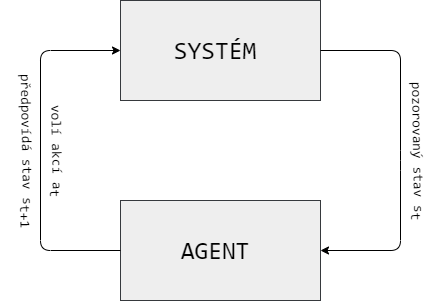
\includegraphics[scale=0.5]{system}
	\centering
	\caption{Uzavřena smyčka}
\end{figure}

\par Protože se jedna o systému s určitou mírou nejistoty nelze jednoznačně předpovědět, který stav nastane jako další. Avšak můžeme odhadnout pravděpodobnost přechodu k dalšímu pozorovanému stavu. Model, který odhaduje tuto pravděpodobnost přechodu nazýváme prediktor a značíme $f(.\mid .)$ (angl. forecaster). K matematickému popisu tohoto  problému se používá diskrétní markovský rozhodovací proces, který poskytuje matematický rámec pro modelování rozhodování v situacích, kdy jsou výsledky zčásti náhodné a zčásti pod kontrolou uživatele.


\textbf{Definice 1.1:} Diskrétní markovský rozhodovací proces je uspořádaná čtveřice\\ $(S,A,P(\cdot ,\cdot ),R(\cdot ,\cdot ))$, kde
\begin{itemize}
	\setlength\itemsep{0em}
	\item{$S$ je konečná množina stavů,}
	\item{$A$ je konečná množina akcí,}
	\item{$f(s \mid a, s')=\Pr(s_{t+1}=s \mid a_t = a, s_{t}= s')$ je pravděpodobnost, že akce $a$ ve stavu $s'$ v čase $t$ povede v čase $t+1$ do stavu $s$,}
	\item{$R(s\mid a, s')$ je okamžitý užitek dosažený po přechodu stavu na $s$ ze stavu $s'$ s pravděpodobností přechodu $P(s \mid a, s')$.}
\end{itemize}

Tato práce slouží pro libovolné $R$ a jeho konkrétní volba není pro tuto práci důležitá.
Jak bylo zmíněno dřív, většina systému, na kterých potřebujeme provést rozhodování a následné předpovídání je nejista a tyto pravděpodobnosti přechodů nejsou známé. Na základě prediktoru $f_t(s_{t+1} \mid a_t, r_t)$ agenta odhaduje pravděpodobností přechodu k dalšímu pozorovanému stavu $s_{t+1}$ za podmínky zvolené akce $a_t$ a regresnímu vektoru $r_{t}$. Odhadování provedeme pomocí bayesovské statistiky podle teorii v BP. V sekci 1.2. nasleduje souhrn důležitých předpokladů a odvozených vět, které jsou relevantní i pro tuto práci. 

\section{Bayesovské odhadování parametrů}
K dobrému rozhodování je potřeba předpovídat jak se chová systém, ve kterém rozhodování provádíme. To znamená předpovídat jaký stav nastane po určité akcí v daných podmínkách. V případě, že předpovíme chování systému s dobrou přesnosti můžeme vybrat, jakou posloupnost stavů preferujeme a na základě toho vybrat potřebnou akcí. Předpokládáme, že posloupnost stavů z množiny stavů $S = \{s_1, s_2, \dots s_n \}$ a posloupnost akcí z množiny $A = \{a_1, a_2, \dots a_m \}$ jsou agentovi známy v určitém čase t. K předpovědi dalšího stavu chceme zjistit souvislosti mezi předešlými stavy S a akcemi A, nazývané pravděpodobnosti přechodu, resp. prediktory $f(s_t, a_t \mid s_{t-1}, a_{t-1}, ..., s_1)$ v určitém čase $t$.

Prediktor $f$ je nejprve parametrizován parametrem $\theta \in \Theta$. Tato závislost je popsána jako $f(s_t, a_t \mid r(t-1), \theta)$, díky čemuž se zužuje odhad $P$ jenom na odhad parametru $\theta$. Při bayesovském přístupu považujeme parametr $\theta$ za náhodnou veličinu, jejíž hodnotu sice nepozorujeme, ale jejíž rozdělení považujeme za známé.
Agent používá parametrický model $m(s_t \mid a_t, r(t-1)) = \Theta_{s_t\mid a_t,r_{t-1}}$, který schovává odhady neznámého (multivariančnímu) parametru $\theta$ na základě .... 
\textcolor{red}{Ted nerozumim co je model}
Pomocí řetězového pravidla a vlastnostem marginální pravděpodobnosti lze pojmout prediktor jako:
\begin{eqnarray}
	f_t(s_t, a_t \mid r(t-1)) = 
	\int_{\Theta} m_t(s_t \mid a_t, r(t-1), \theta) p(a_t \mid r(t-1), \theta)p_{t-1}(\theta)d\theta.
\end{eqnarray}

$p(a_t \mid r(t-1), \theta)$ je generátor akcí a řídí se agentem. Agent vybírá akci, která bude ovlivňovat systém, proto generátor akcí nezná parametry systému. Pro něj platí tzv. přirozené podmínky řízení.

\par \textbf{Předpoklad 1.6: }\textit{(Přirozené podmínky řízení)} Pokud agent současně sleduje a řídí systém, pak jeho rozhodnutí (akce), neposkytují žádné další informace o stavu systému a naopak. A platí:

\begin{equation}
	P(a_t \mid r(t-1), \theta) = P(a_t \mid r(t-1)).
\end{equation}

Aposteriorní hustota pravděpodobnosti $p(\theta \mid r(t-1))$ kvantifikuje znalosti agenta nashromážděné až do času $t-1$. Po pozorování další časové smyčky a získaní dalšího pozorovaného stavu agent aktualizuje aposteriorní hustotu pravděpodobností pomocí Bayesova pravidla:
\begin{equation}
	p_t(\theta) = \frac{m_t(s_t \mid a_t, r(t-1), \theta)p_{t-1}(\theta)}{\int_{\Theta} (m_t(s_t \mid a_t, r(t-1), \theta)p_{t-1}(\theta)d\theta} 
\end{equation}
$p_0(\theta)$ je apriorní hustotu pravděpodobnosti veličiny $\theta$. Tato hustota pravděpodobnosti vyjadřuje apriorní informaci o možných hodnotách parametru $\theta$. Může být zvolena zcela objektivně, např. na základě zkušenosti s pozorováními z minulosti nebo na základě vnějších informací, např. z fyzikální podstaty problému. Možná je ale také subjektivní volba vyjadřující individuální názor na pravděpodobnosti výskytu jednotlivých hodnot parametru.

\par \textbf{Předpoklad 1.2} Předpokládáme, že zkoumaný systém má konečnou paměť $p\in N$, což znamená, že model $m_t(s_{t} \mid  a_{t},r(t-1)) = m_t(s_{t}\mid a_{t},r_{t-1},\ldots,r_{t-p})$ závisí na p posledních stavech a akcích systému.

Za předpokladu konečné paměti jsou pravděpodobnostní funkce přechodu tabulky konečného rozměru. Takovou tabulku si můžeme představit jako vícerozměrné pole, jehož rozměr závisí na počtu regresorů. Neznámé, dle předpokladu časově neproměnné hodnoty jejich prvků, tvoří neznámý (mnoharozměrový) parameter $\theta$. V jistém stavu $s_{t}=s$ při jisté podmínce $a_{t}=a$ a $r_{t-1}=r$ z pravděpodobnostní tabulky odhaduji jistou hodnotu $\theta_{s \mid a,r}$, která musí být nezáporná a součet přes předpovídané stavy musí být jedna. 
Pak můžeme vyjádřit apriorní hustotu pravděpodobnosti pomocí následujícího výrazu:

\begin{equation}
	p_t(\theta) \propto \prod_{{s},{a},{r}} \theta_{s \mid a, r}^{ \sum_{k=1}^t\delta(s, s_k)\delta(a, a_k)\delta(r, r_{k-1})}p_0(\theta).
\end{equation}
\\*
Značíme pomocnou funkci (statistiku):
\begin{equation}
	V_t(s, a, r) = V_{t-1}(s, a, r) + \delta(s, s_t) \delta(a, a_t) \delta(r, r_{t-1}).
\end{equation}
Tato funkce (statistika) vyjadřuje počet cest $r \rightarrow a \rightarrow s$, které jsme dostali během pozorování do času t.
Apriorní pravděpodobnost $P(\theta)$ vyjadřuje znalost o systému před počátkem sledování. Tuto znalost můžeme vyjádřit jako počáteční hodnotu statistiky $V_0(s, a, r)- 1$.
Potom apriorní hustotu pravděpodobnosti lze vyjádřit pomocí následující věty:

\par \textbf{Věta 1.3} Pro systém s konečným počtem regresorů je aposteriorní hustota pravděpodobnosti $P(\theta \mid s_t, a_t, r_{t-1})$ v určitém čase $t$ ve tvaru:

\begin{equation}
	P(\theta \mid s_t, a_t, r_{t-1}) = \frac{\prod_{{s}, {a}, {r}} \theta_{s \mid a, r}^{ V_t(s, a, r) + V_0(s, a, r)- 1}}{\int_{\Theta} \prod_{{s}, {a}, {r}} \theta_{s \mid a, r}^{ V_t(s, a, r) + V_0(s, a, r)- 1}d\theta },
\end{equation}
kde množina $\Theta$ je definována jako: 
\begin{equation}
	\Theta=\left\{\theta = (\theta_{s|a,r})_{s\in S,a\in A,r\in R}:\,\theta_{s|a,r}\geq 0, \sum_{s\in S}\theta_{s|a,r}=1\ \mid \forall a\in A,r\in R  \right\}.
	\nonumber
\end{equation}

Potom integrační obor $\Theta$ je složitý simplex, díky čemuž jsou integrály beta funkce statistik parametrizujících integrovanou funkci. 

Model agenta pak lze zapsat jako $m_t(s_t \mid a_t, r_{t-1}, \theta) = \theta_{s \mid a, r}^{ V_t(s, a, r)} $

\par \textbf{Věta 1.4:} Pro systém s konečným počtem regresorů lze pravděpodobnost přechodu ke stavu $s_t = s$ za podmínky akce $a_t = a$ a regresního vektoru $r_{t-1} = r$  a nasbírané statistiky $V = V_{t-1} + V_{0}$ vypočítat jako:
\begin{equation}
	P(s \mid a,  r, V) = \frac{V_{s \mid a, r}}{\sum_s V_{s \mid a, r}}.
\end{equation}

Podle této věty platí, že pravděpodobnost přechodů není nic jiného než počet posloupnosti dělený na pozorovanou četnost trojic ($s,a,r$) (opravenou apriorními představami) pro každý předpovídaný stav, což připomíná klasicky výpočet pravděpodobnosti.


\section{Kombinace prediktorů}

K dobrému předpovídaní chování složitých systému je potřeba velké množství pozorování a analyzovaní. Složité systémy s velkým množstvím různých stavu, akcí a jejích souvislosti požadují velký počet pozorování pro přesné odhadování. Často se dostaneme do situaci, když je vhodný a přínosný použit nějakou další informací o systému, která je odlišná od informací získaných pomocí našeho prediktoru. Tyto informace mohou být ve formě námi provedených měření na námi modelovaném systému, měření provedených v modelu podobného charakteru nebo měření provedená někým jiným. Zjednodušeně to můžeme popsat jako spojení svých dat s daty nějakého poradce, který má další zkušenosti s chováním daného nebo podobného systému a má svojí představu o pravděpodobnosti dalšího stavu pro danou historii. Potom rozšíříme svá data pomocí této informace a tím zlepšíme předpovídání. Tato informace může být pro náš model pravdivá pouze částečně, protože měření zdánlivě podobného systému může být zcela odlišné od našeho systému.


Informací, kterou získáme souhrnně nazveme externí i když praktický tyto data byt externí nemusejí. Může je jednat například o víc naších prediktoru, které sledujeme podle různých regresorů [BP].   
Tato informace ani v tomto případě nemusí byt úplně pravdivá, například protože zkoumaný systém nezávisí nebo závisí jenom částečně na regresorech, které tento prediktor sleduje. 

Otázkou, kterou se budeme zabývat je jakým způsobem kvantifikovat míru platnosti externí informace pro náš model, tato hodnota bude reprezentována tzv. váhou důvěry.

\textbf{Definice 1.5:} Váhou důvěry budeme nazývat parametr představující důvěru v k-tou externí informaci $e_k$. Tento parametr budeme značit $v_k$. 

\textbf{Poznámka 1.6:} Předpokládáme, že váha důvěry je diskrétní veličina a budeme ji volit tak, aby splňovali následující podmínky:
\begin{equation}
	v_i \in \textbf{v} = \{v_1, v_2, ...v_n\}, n \in \mathbb{N}, n < \infty, \sum_{i=1}^n b(v_i) = 1 
\end{equation}
kde $b(v_i)$ je pravděpodobnost toho, že váha $v_i$ přivede k nejlepšímu odhadu parametru $\theta$.

Druhou související otázkou je jak spojit informace námi provedenými měřeními s externími informacemi. Předpovídací model agenta $m_t(s_t \mid d(t-1))$ chceme rozšířit nějakou externí informací $k$ ohledně chování pozorovaného systému. Předpokládáme, že tyto data jsou v podobném tvaru jako data, která chceme doplnit.
Například můžou být získaná pomocí jeho vlastního předpovídacího modelu $e_t()$, který je vypočítán nezávisle na agentovi a má svojí představu o pravděpodobnosti dalšího stavu pro danou historii chování akcií. 
V každém cyklu, ve kterém externí informaci dostaneme obnovíme aposteriorní hustotu pravděpodobnosti agenta sloučením modelu agenta s modelem poradce s nastavením odpovídající váhy důvěry $v_k$ na základě následující věty:  

\textbf{Věta 1.7: } Nechť platí, že $m_t(s_{t+1} \mid a_{t+1}, r_t, \theta)$ je parametrický model systému, $e_{k,t}$ je hustota pravděpodobnosti přidávaných dat, $v_k \geq 0$ je jejich váha důvěry. Pak platí, že aposteriorní hustotu pravděpodobnosti $p_t(\theta)$ lze spočítat jako: \\
\begin{equation} p_t(\theta ) \propto p_{t-1}(\theta)\exp\{v\int_{s} e_t(s \mid z_{t+1})\ln(m(s \mid a_{t+1}, r_t, \theta))\}.
	\nonumber
\end{equation}

$e_t(s \mid z)$ je externí model poradce operující na svém regresoru z, tj $e_t(s_{t+1} \mid a_{t+1}, r_t) = M(s_{t+1} \mid z_{t+1})$. Obecně $z_{t+1}$ odpovídá situaci, kdy agent užívá $a_{t+1}, r_t$. Potřebujeme-li to zdůraznit píšeme místo z symbol $z(a; r)$.

V diskrétním případě pro systém s konečnou paměti model poradce $e_k$ podle věty 1.4 můžeme představit ve tvaru:
\begin{equation}
	\centering
	e_{t,k}(s \mid a,r)= \frac{W_{s|z}}{\sum_{s\in \textbf{s}}W_{s|z}},
	\nonumber
\end{equation}
kde $W_{s \mid z}$ = počet pozorovaných hodnot (s, z = z(a, r)) vyskytujících se současně s
výskyty (s, a, r) zvětšený o apriorní statistiku, kterou užil poradce.
\\*
Pak slučovaní modelu agenta s k-tou externí informací můžeme spočítat pomocí věty (BP): 


\textbf{Věta 1.8:} Pro systém s konečným počtem stavu lze slučovaní k-té externí informaci $e_k$ pro výpočet aposteriorní hustoty pravděpodobnosti $p_t(\theta) $ v čase t provést jako:
\begin{equation}
	p(\theta) \propto \prod_{{s},{a},{r}}
	\theta_{s|a,r}^{V_{t}(s,a,r)+V_{0}(s,a,r)-1+v\frac{W_{t}(s, z(a,r))}{\sum_{s}W_{t}(s, z(a,r))}}.
	\nonumber
\end{equation}

Slučovaní parametrického modelu postupně provedeme s každou externí informaci a díky tomu dostaneme novou
aposteriorní pravděpodobnost parametrů modelu, který používá agent pro opravování svého prediktoru f.



\section{Minimální expected relative entropy principle}

\textbf{Definice 1.9:} Jsou-li spojité p a q pravděpodobnostní míry nad množinou X a je-li P absolutně spojitá míra vzhledem ke q, tak je Kullbackova–Leiblerova divergence P od Q definována jako:
\begin{equation}
	D(P \mid\mid Q) = \int_{x} p(x) \ln(\frac{p(x)}{q(x)}dx
\end{equation}

Kullbackova–Leiblerova divergence $D(P \mid\mid Q)$ nabývá hodnoty nula, právě když se distribuce P a Q rovnají skoro všude; v opačném případě je divergence kladná.


\begin{equation}
	p^0 \in Arg \min_{p \in {p}} D(P \mid\mid P_0) = Arg \min_{p \in {p}} \int_{x} P(X) \ln(\frac{P(X)}{P_0(X)}) 
\end{equation}


\chapter{Popis a řešení problému}

\section{Formulace a navrh řešení problému}

Nechť máme nějakou ohraničenou část světa - systém, na kterém agent chce provést předpovídaní. V systému máme konečný počet stavů a akcí. Cílem agenta je odhadnout pravděpodobnost výskytu dalšího pozorovaného stavu   
      
- popsat detailne co je problemem meho vyzkumneho ukolu 
- popsat jak ho budu resit 

\section{Odhadování váhy důvěry}


K použiti metody uvedené v přípravné kapitole je potřeba nastavit vhodnou váhu důvěry pro každý model poradce. Pro poradce, který poskytuje důvěryhodnou informaci nastavíme vyšší hodnotu tohoto parametru. Naopak modelu poradce, kterému nevěříme přiřadíme nízkou hodnotu a tím ovlivníme predikci. V důsledku hodnota váhy důvěry má velký vliv na výslednou predikci. 


Dána kapitola se zabývá odhadováním takové váhy důvěry, aby byla zaručena nejkvalitnější předpověď dalšího stavu systému. První část této kapitoly je zaměřena na odhadování váhy důvěry na základě bayesovského odhadovaní v intervalu $ w \in [0; 1] $. Druhá část kapitoly je zaměřena o modifikaci intervalu $ w \in [0; \infty ]$. Třetí část popisuje případ, když váha důvěry k poradcovi se mění v průběhu času.  


\subsection{Odhadování konstantní váhy důvěry}
V této sekcí ukážeme odhadování váhy důvěry pomocí Bayesovské statistiky.
Nejprve budeme předpokládat, že váha důvěry je diskrétní veličina, která leží v intervalu  $ w \in [0; 1] $. Z toho plyne, že ze zavedení \textit{důvěryhodnostního parametru} plynou dva možné krajní případy. Prvním je, že nevěříme externí informaci vůbec, tedy $ w = 0 $, nebo druhý extremální případ, že jí věříme zcela tzn. $ w = 1 $. Z této úvahy nám vyplývá interval možných hodnot parametru $ w $ ve tvaru $ w \in [0; 1] $, ve kterém se \textit{důvěryhodnostní parametr} nachází.

Potřebujeme odhadnout nejenom parametr $\theta$, ale i parametr $w$. Neměnná váha $w$ rozšiřuje parametr $\theta \in \{\Theta\}$ na neznámé $(\theta, w) \in (\Theta, [0, 1])$.

Předpokládáme, že hodnota váhy důvěry je diskrétní veličina. Budeme volit parametry váhy důvěry tak, aby splňovali tyto podmínky:
\begin{itemize}
	\item $w_i \in \{w_1, w_2, \dots , w_n\}$, kde $n < \infty$ a $n \in \mathbb{N}$
	\item $\sum_{i=1}^n P(w_i) = 1$
\end{itemize}

 Hledáme pravděpodobnost $P(w, \theta)$ ve tvaru:

\begin{equation}
P(w, \theta) = P(\theta \mid w) P(w). 
\end{equation}
kde $P(w)$ je apriorní pravděpodobnost, tj pravděpodobnost založena na naší apriorní znalosti o důvěryhodnosti informaci poradce. $P(w \mid \theta)$ je podmíněna pravděpodobnost, že pro konkrétní hodnotu parametru $w$ dostaneme takový parametr $\theta$, který povede k nejlepší předpovědí dalšího stavu.  

Napsat
- jak probiha odhadovani vahy
- jak se zmeni vypocet pravdepodobnosti prechodu
- jak se zmeni vypocet posteriorni pravdepodobnoti a slucovani dat
- jak bude vypadat pravdepodobnost vahy 

\subsection{Odhadování diskrétní váhy důvěry bez intervalu}
- popis proc je to dobry 
- navrh reseni 


\subsection{Váha důvěry, která se mění z časem}
- popis situace 
- bayesova filtrace
- proc ji nepouzivame 
- exponencialni zapominani z knizky
- pro nas pripad  

\chapter{Experimenty}

\pagestyle{headings}

\chapter*{Závěr}

\pagestyle{plain}

\addcontentsline{toc}{chapter}{Záv\v{e}r}

Text závěru....
\begin{thebibliography}{1}
\bibitem{Allen-Cahn}S. Allen, J. W. Cahn: \emph{A microscopic theory
for antiphase boundary motion and its application to antiphase domain
coarsening}. Acta Metall., 27:1084-1095, 1979.

\bibitem{CINECA}G. Ballabio et al.: \emph{High Performance Systems
User Guide}. High Performance Systems Department, CINECA, Bologna,
2005. \url{www.cineca.it}

\bibitem{rumpf3}J. Becker, T. Preusser, M. Rumpf: \emph{PDE methods
in flow simulation post processing}. Computing and Visualization in
Science, 3(3):159-167, 2000.
\end{thebibliography}

\end{document}
